\newpage
\subsection{Precision Placement Test}

\paragraph{Purpose and Focus of the Test}
The purpose of the \iaterm{Precision Placement Test}{PPT} is to assess the robot’s ability to grasp and place objects into object-specific cavities. This demands advanced perception abilities (to recognize the correct cavity for each object) and manipulation abilities (to grasp and place the object in such a manner that it fits into the cavity).

\paragraph{Scenario Environment}
The same arena as for the Basic Manipulation Test is used (Figures 5.4 and 5.5) whereas the plane of one service arena includes object-specific cavities as shown in the Figure 6.3 and Figure 6.4. For each object used in the test there will be one specific cavity. The cavity has the dimension of the object plus a 2 mm offset for each dimension. At most five cavities are used in the test.


\begin{figure} [h!]
\begin{center}
\subfloat[F20\_20]{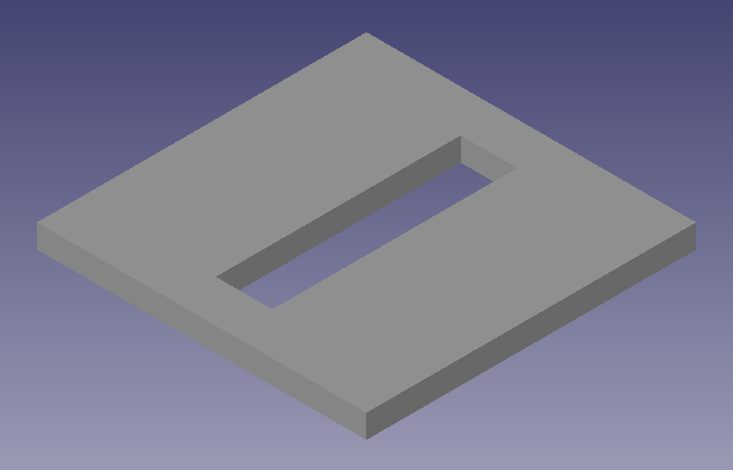
\includegraphics[width = 2cm]{../images/ppt_F20.png}}
\subfloat[S40\_40]{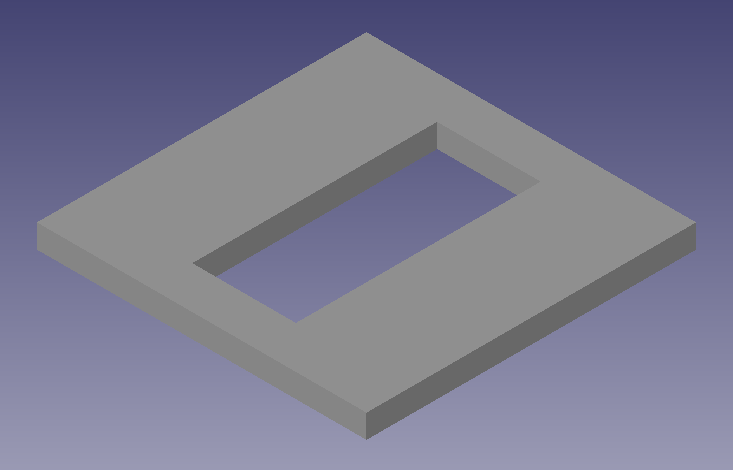
\includegraphics[width = 2cm]{../images/ppt_S40.png}} 
\subfloat[M20\_100]{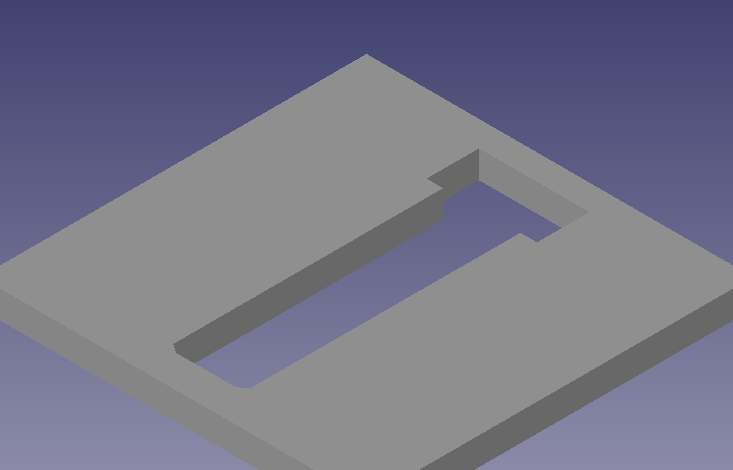
\includegraphics[width = 2cm]{../images/ppt_M20_100.png}} \\
\subfloat[M20]{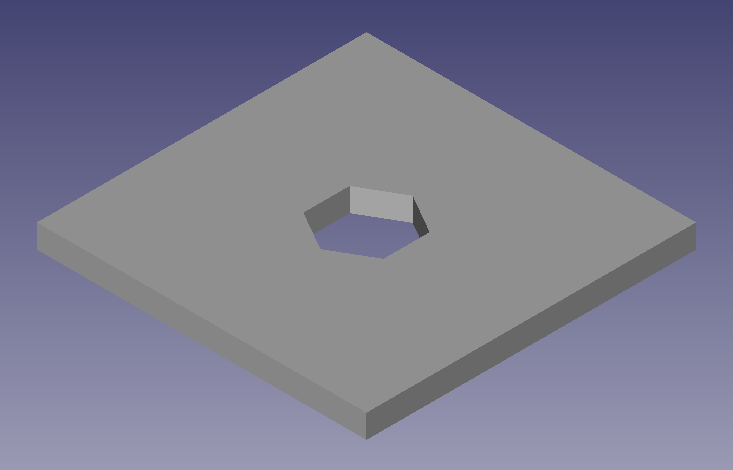
\includegraphics[width = 2cm]{../images/ppt_M20.png}}
\subfloat[M30]{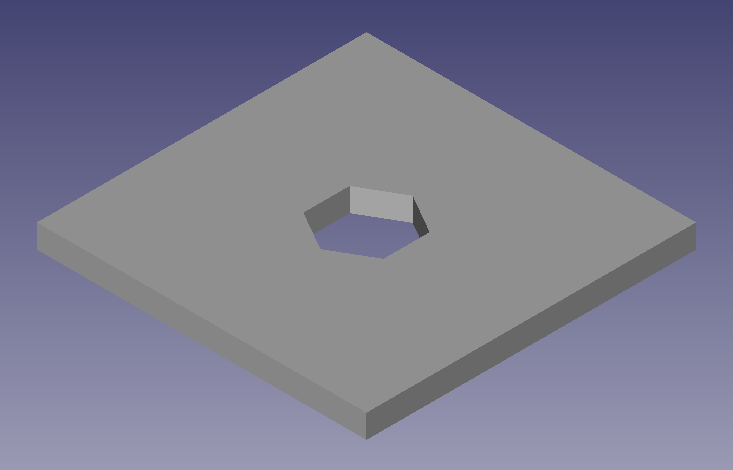
\includegraphics[width = 2cm]{../images/ppt_M30.png}} 
\subfloat[V20, R20]{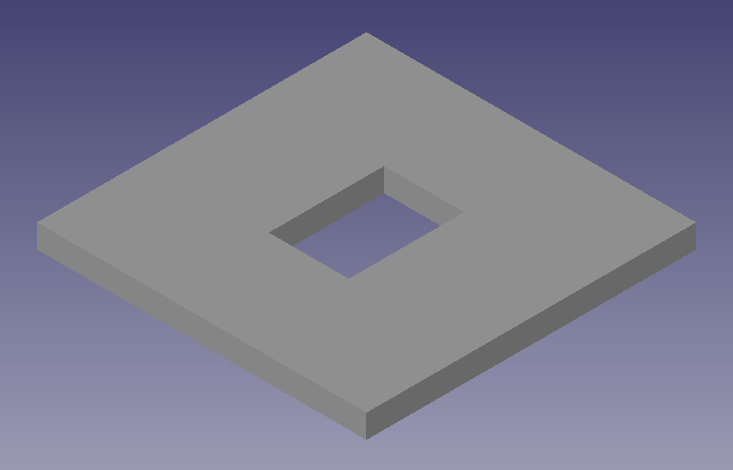
\includegraphics[width = 2cm]{../images/ppt_VR20.png}} 
\end{center}
\caption{Illustration of horizontal cavities for the different kind of objects}
\label{fig:ppt_vertical_tiles}
\end{figure}


\begin{figure} [h!]
\begin{center}
\subfloat[F20\_20]{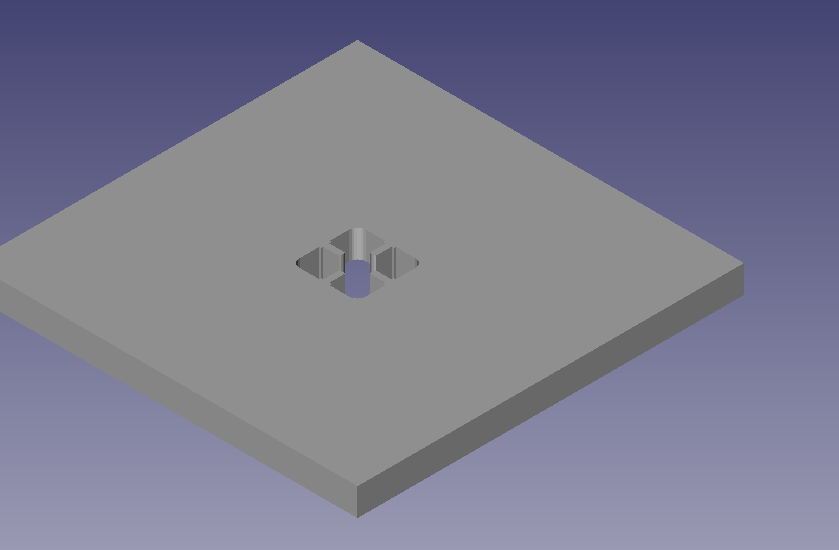
\includegraphics[width = 2cm]{../images/ppt_F20_v.png}}
\subfloat[S40\_40]{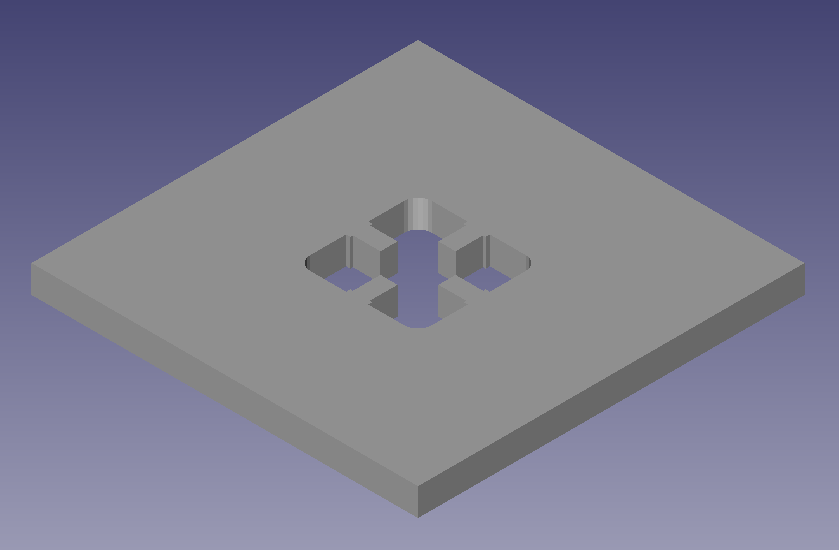
\includegraphics[width = 2cm]{../images/ppt_S40_v.png}} 
\subfloat[M20\_100]{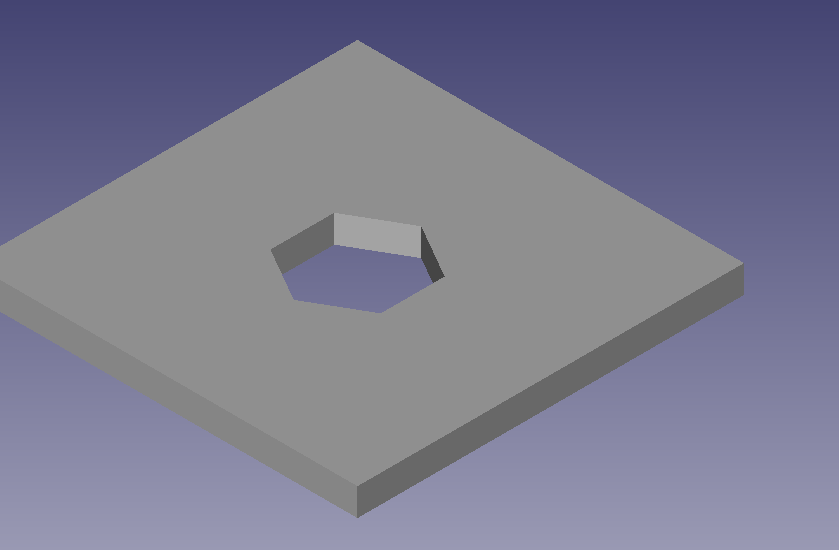
\includegraphics[width = 2cm]{../images/ppt_M20_100_v.png}} \\
\subfloat[M20]{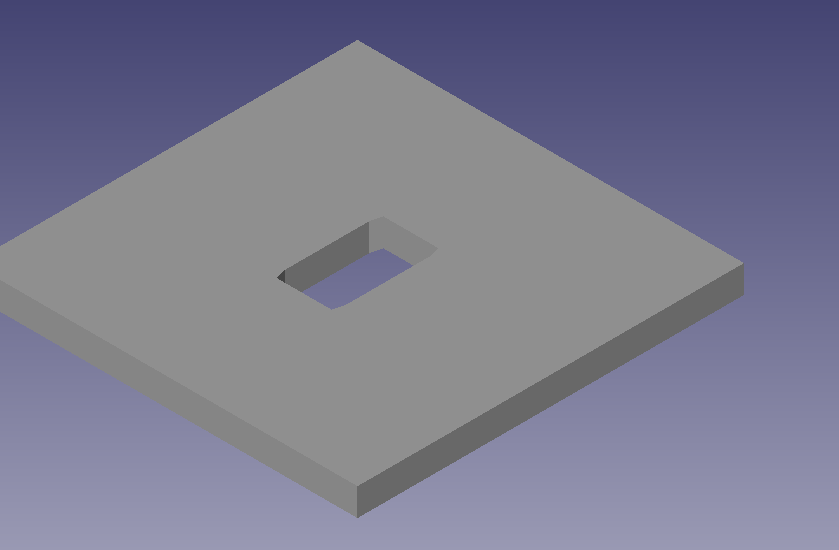
\includegraphics[width = 2cm]{../images/ppt_M20_v.png}}
\subfloat[M30]{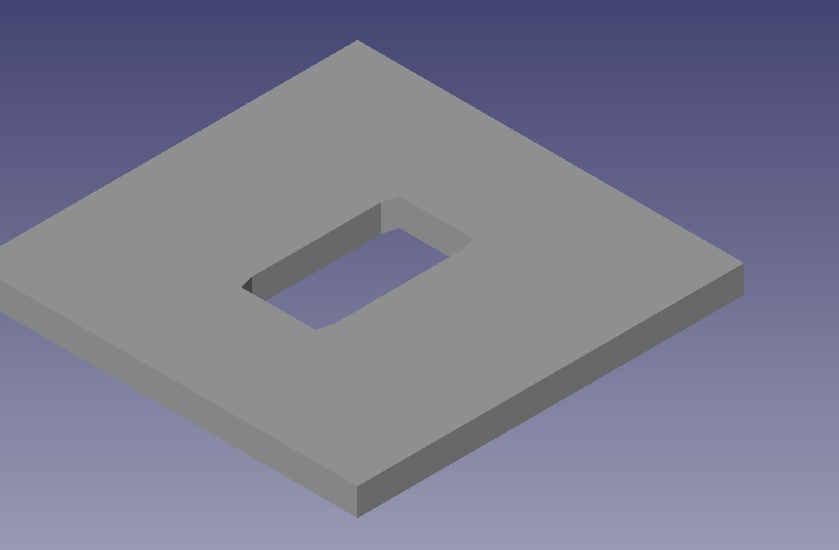
\includegraphics[width = 2cm]{../images/ppt_M30_v.png}} 
\subfloat[V20, R20]{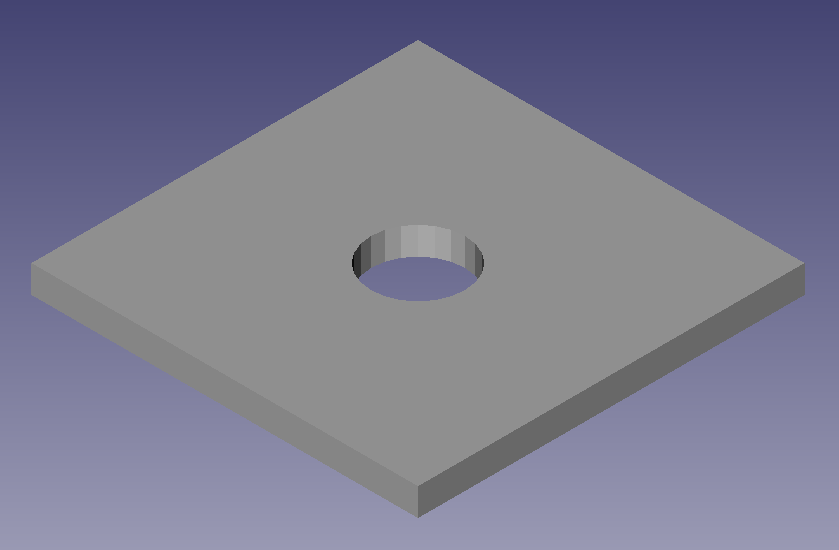
\includegraphics[width = 2cm]{../images/ppt_VR20_v.png}} 
\end{center}
\caption{Illustration of vertical cavities for the different kind of objects}
\label{fig:ppt_horizontal_tiles}
\end{figure}

\paragraph{Manipulation Objects}
The same manipulation objects as for the Basic Manipulation Test are used. 

\paragraph{Task}
A single robot is used. The robot is placed by the team freely within the arena. The objective of the task is to pick the object which is placed in this service area and make a precise-placement in the corresponding cavity at the service area with the special PPT platform (an example configuration is illustrated in Figure \ref{fig:ppt_plattform}). 

\begin{figure}
\centering
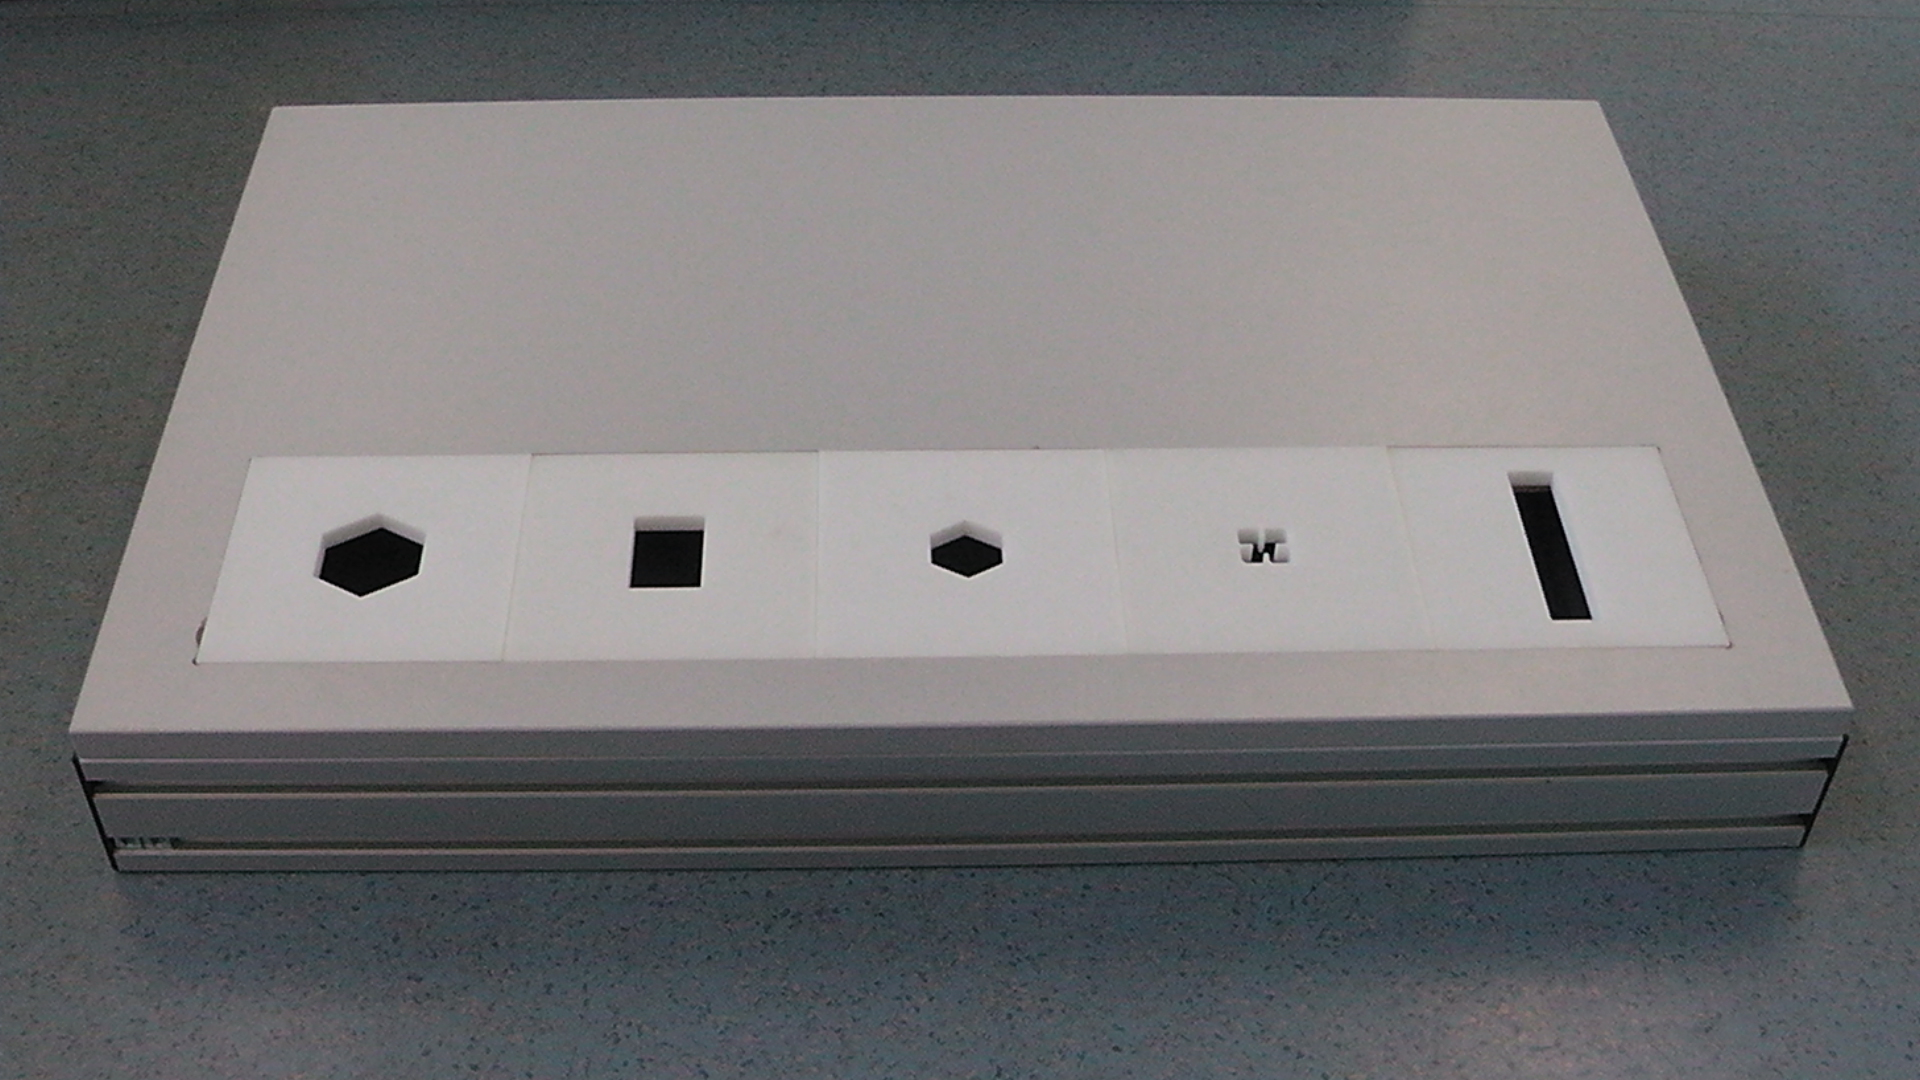
\includegraphics[width=0.6\textwidth ]{../images/ppt_plattform.jpg}
\caption{The PPT platform including five cavity tiles}
\label{fig:ppt_plattform}
\end{figure}

The task consists of multiple grasp and place operations, possibly with base movement in between, which will, however, be short. The set of objects which are used in the test is known a priori (at most the number of objects specified in Section 5.5.1). The task is finished once the objects are picked up and placed in corresponding cavities or when the time foreseen for the run ends. Note that the placement of the object in the cavity is finished when the object is fallen into the cavity (i.e. at least some part of the object has to touch ground floor underneath the cavity).
\par
All objects to be transported in a run of a team and the corresponding cavities share the same orientation, either horizontal or vertical. This may vary between different teams and different runs.
\par
An example task specification is given here:
\par
PPT\textless S1,(M20, S40\_40\_G),S2\textgreater
\par
where S1 is the location where to pick up the objects M20 and S40\_40\_G. The objects need to be placed then in the corresponding cavities at location S2.
%
%\subsection{Complexity Levels}
%
%All Complexity Options from BMT apply.
%
%\subsubsection{PPT Orientation Complexity (bonus factor = 0.2):}
%The cavities can be placed in all orientations.
%\subsubsection{PPT Rotation Complexity (bonus factor = 0.2):}
%The cavities can be placed in all orientations.

\paragraph{Rules}
The following rules have to be obeyed:

\begin{itemize}

\item The order in which the teams have to perform will be determined by a draw.
\item A team has a time period of 8 minutes to complete a run.
\item At the beginning of a team’s period, the team will get the task specification. 
\item A manipulation object counts as successfully grasped as specified in Section 5.5.3.
\item An object counts as placed correctly if it fell through the correct cavity and touches the ground beyond. It may happen that an object blocks the cavity for the next object, e.g. by standing upright on the floor. In that case a referee may remove that object (which remains to count as a successful drop). If the referee is not able to do so and the robot places another object into the blocked cavity, it counts as a correct placement if it would have been successful without the blocking object.
\item The time is stopped when the robot has placed the last object correctly. If a team cannot complete the task within the specified time, the run will be stopped after it is exceeded.  

\end{itemize}

%\subsection{Scoring}
%Points are awarded as follows:
%
%\begin{itemize}
%\item 50 points are awarded for successfully grasping an object.
%\item 100 points are awarded for successfully placing a manipulation object into the correct cavity.
%\item 50 points are awarded if the task specification has been completely fulfilled. The task is considered as fulfilled if all objects have been dropped in the right cavity. The robot does not have to leave the arena.
%\item a penalty of -50 points is given for each object which has been dropped into the wrong cavity
%\item The reached points of a test will be multiplied with a defined complexity factor depending on the previously chosen complexity level.
%\end{itemize}


